\documentclass[twocolumn,9pt]{jsproceedings}
\RequirePackage[l2tabu,orthodox]{nag}  % 古いコマンドやパッケージを使用した場合に警告する
%\usepackage{subcaption}
\usepackage[all,warning]{onlyamsmath}  % amsmath が提供しない数式環境を使用した場合に警告する
% \usepackage{flushend}  % 最終ページの2カラムの左右の高さを揃える
\usepackage{here} %図の場所の指定で[h](ここに貼る)を指定するためのパッケージ
\usepackage[dvipdfmx]{graphicx} %dvipdfmxはjpgやpngの張り込みのために使用
%\usepackage{graphicx}

% タイトル
\title{新卒だけどつくばチャレンジ出るよチームの\\つくばチャレンジ2024での取り組み}

\author{○池邉 龍宏\authorrefmark{1}、海老田 そら\authorrefmark{1}、春山 健太\authorrefmark{1}、大澤 来実\authorrefmark{1}\\森下 敢太\authorrefmark{1}、
深谷 和俊\authorrefmark{1}、藤江 謙伸\authorrefmark{1}、新宮 義規\authorrefmark{1}}

\etitle{Our Team's Efforts in Tsukuba Challenge 2024 as New Graduate Participants}

\eauthor{○Tatsuhiro IKEBE\authorrefmark{1}、Sora EBITA\authorrefmark{1}、Kenta HARUYAMA\authorrefmark{1}、Kurumi OSAWA\authorrefmark{1}\\Kanta MORISHITA\authorrefmark{1}
Kazutoshi FUKAYA\authorrefmark{1}、Kenshin FUJIE\authorrefmark{1}、Yoshiki SHINGU\authorrefmark{1}}

\affiliation{新卒だけどつくばチャレンジ出るよ}

\begin{document}
\maketitle

\authorreftext{1}{社会人}
% \eauthorreftext{1}{Department of Advanced Robotics、Faculty of Advanced Engineering、Chiba Institute of Technology}

% 本文
\section{緒言}

新卒だけどつくばチャレンジ出るよチームは,
同じ会社内にてつくばチャレンジに参加したいという
意志のあるメンバーが集まったチームである。
% チームメンバーは2024年に新規学卒者(新卒)の計8名のメンバー構成で作成された。
% 過去につくばチャレンジに参加したことがある方や初めて参加する方がそれぞれ在籍している。
チームメンバーは2024年に新規学卒者(以下、新卒)の計8名であり、
つくばチャレンジの参加経験は初参加から複数年まで様々である。

本チームの参加目的は、
新卒においても、つくばチャレンジに参加することが可能であることを証明することである。
また本チームの活動を元に、来年のつくばチャレンジで新卒として参加するチームが増えるようにしていきたいと考えている。
% この目的を達成するために各目標を
この目的を達成するために、本チームでは以下を目標と定めた。
\begin{itemize}
  \item[1] 参加登録
  % \item[2] 作成した機体の車検を通す
  \item[2] 独自設計したロボットでの車検合格
  % \item[3] 機体から得られたセンサ情報を用いた事前地図作成
  \item[3] ロボットに搭載されたセンサから得られる情報から歪みの無い地図を取得
  \item[4] 確認走行区間を完走
\end{itemize}
% とした。


本稿では、目標に対する取り組みと結果について説明する。
本稿の構成は次の通りである。
1章では、参加メンバーおよび、参加目的と目標について述べた。
2章ではロボットのソフトウェア、ハードウェア構成について説明し、
3章では本走行の結果と見つかった課題を示す。
% 4章では本年度のつくばチャレンジで利用しなかった研究室での取り組みを紹介し、
4章では本年度のつくばチャレンジで利用しなかった本チームでの取り組みを紹介し、
5章では結言を述べる。

\section{ロボットの構成}

\subsection{概要}
本チームでは、新卒がつくばチャレンジに参加できるようできるだけ安価で開発環境を整えやすいロボット
構成を目指してハードウェアの選定を行った。
\ref{sub:hardware}節では、採用したロボット、センサ、ロボット保護カバーなどの詳細について述べる。

ソフトウェアについては、本チームはROS 2\cite{ROS 2}をベースに構築した。
ソフトウェアの特徴について、\ref{sub:software}節以降で説明する。


\subsection{ハードウェア構成}\label{sub:hardware}
ロボットの外観を図\ref{fig:trainee}に示す。
本ロボットは、ODrive社製の既製品である、BotWheel Explorer Kit\cite{RTshop}がベースになっている。

\begin{figure}[h]
  \begin{center}
    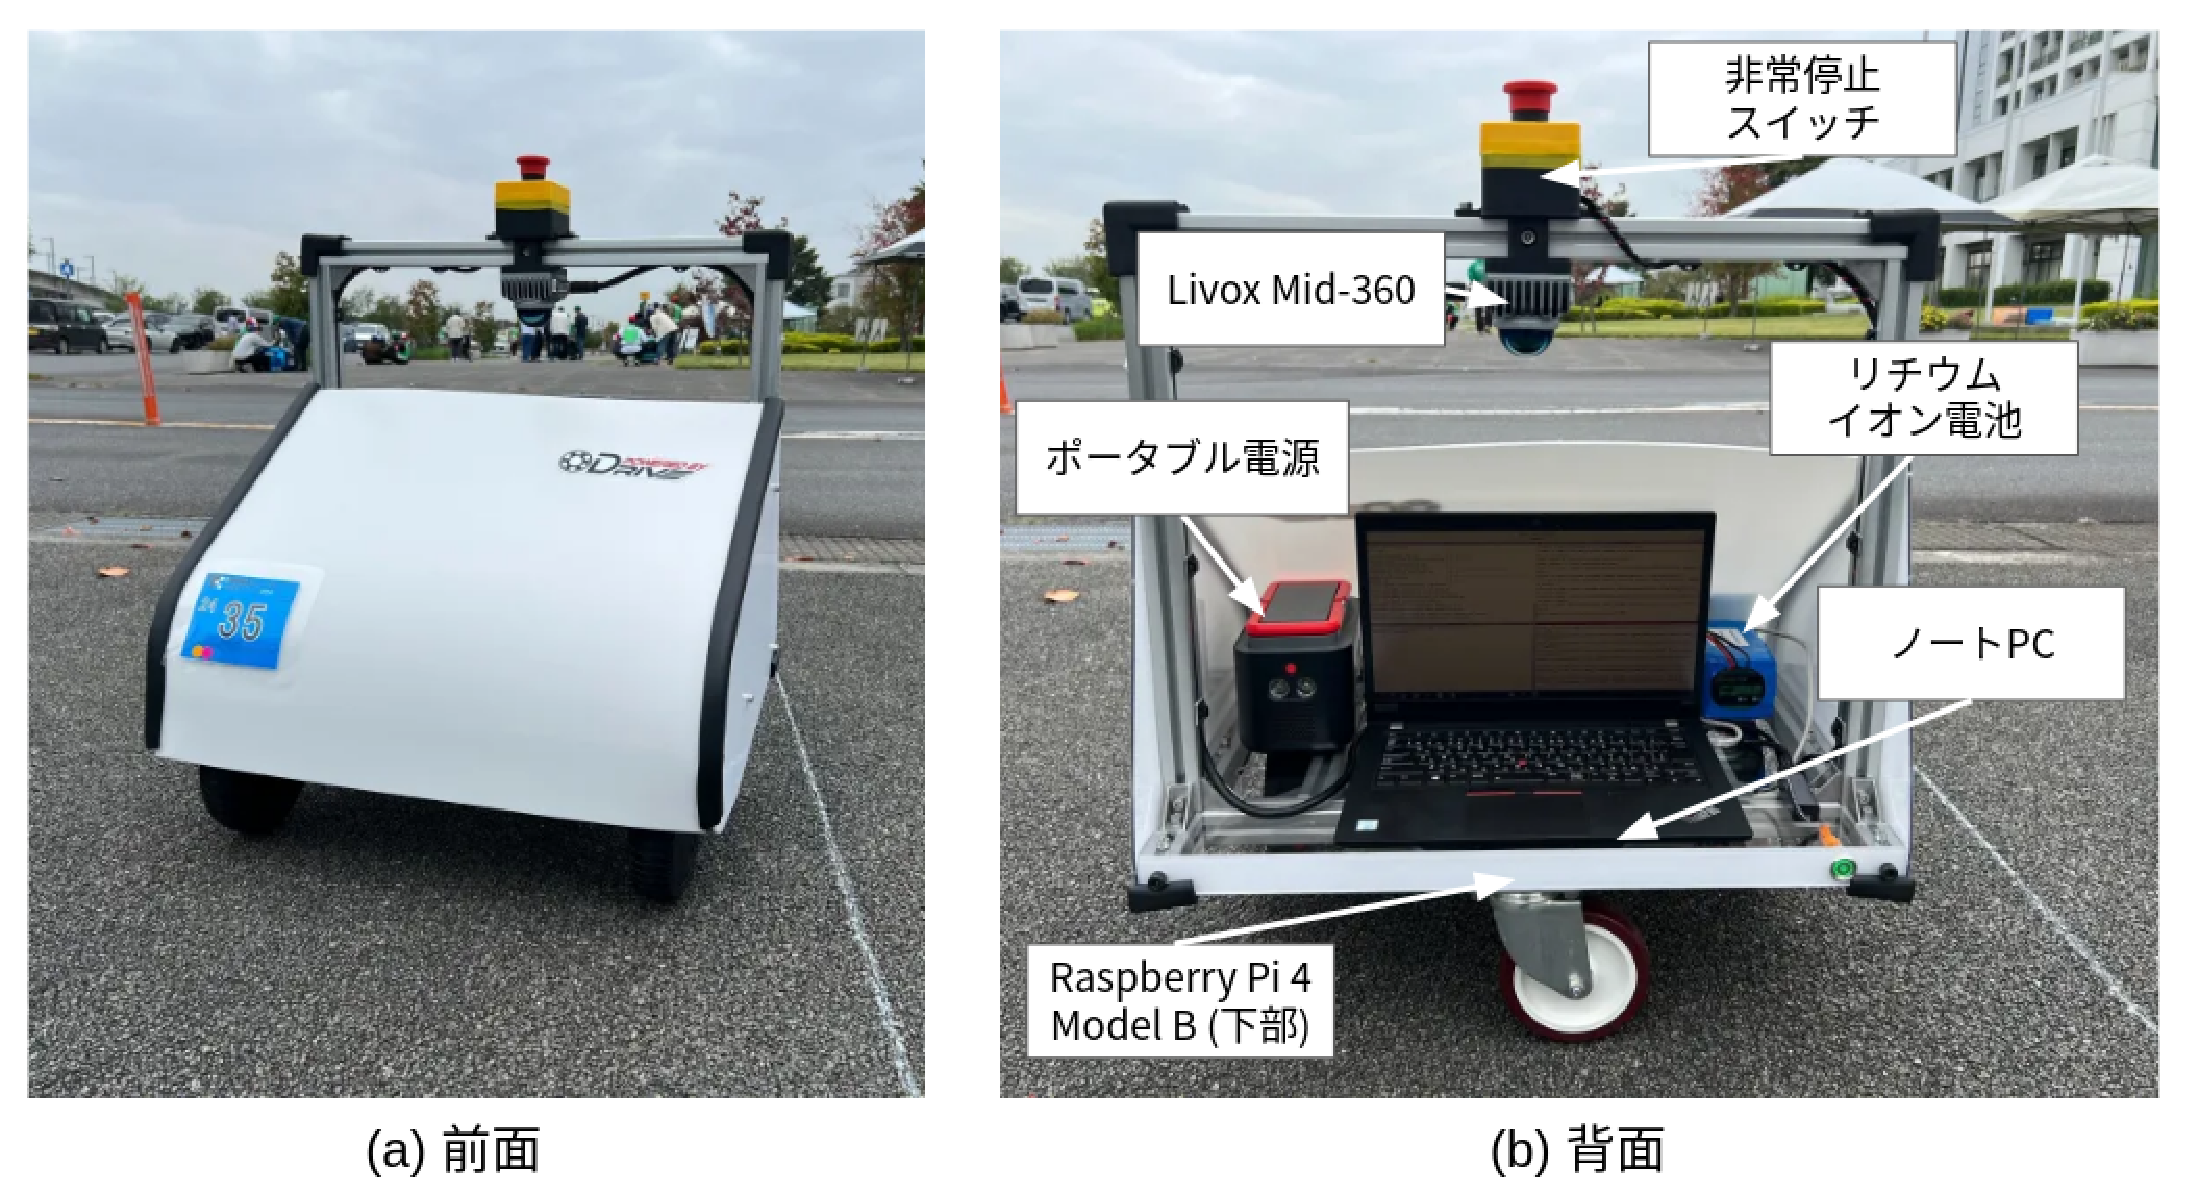
\includegraphics[width=1.0\linewidth]{figs/trainee.pdf}
    \caption{チームの機体(機体名: トレーニー)}
    \label{fig:trainee}
  \end{center}
\end{figure}

\begin{figure}[h]
  \begin{center}
    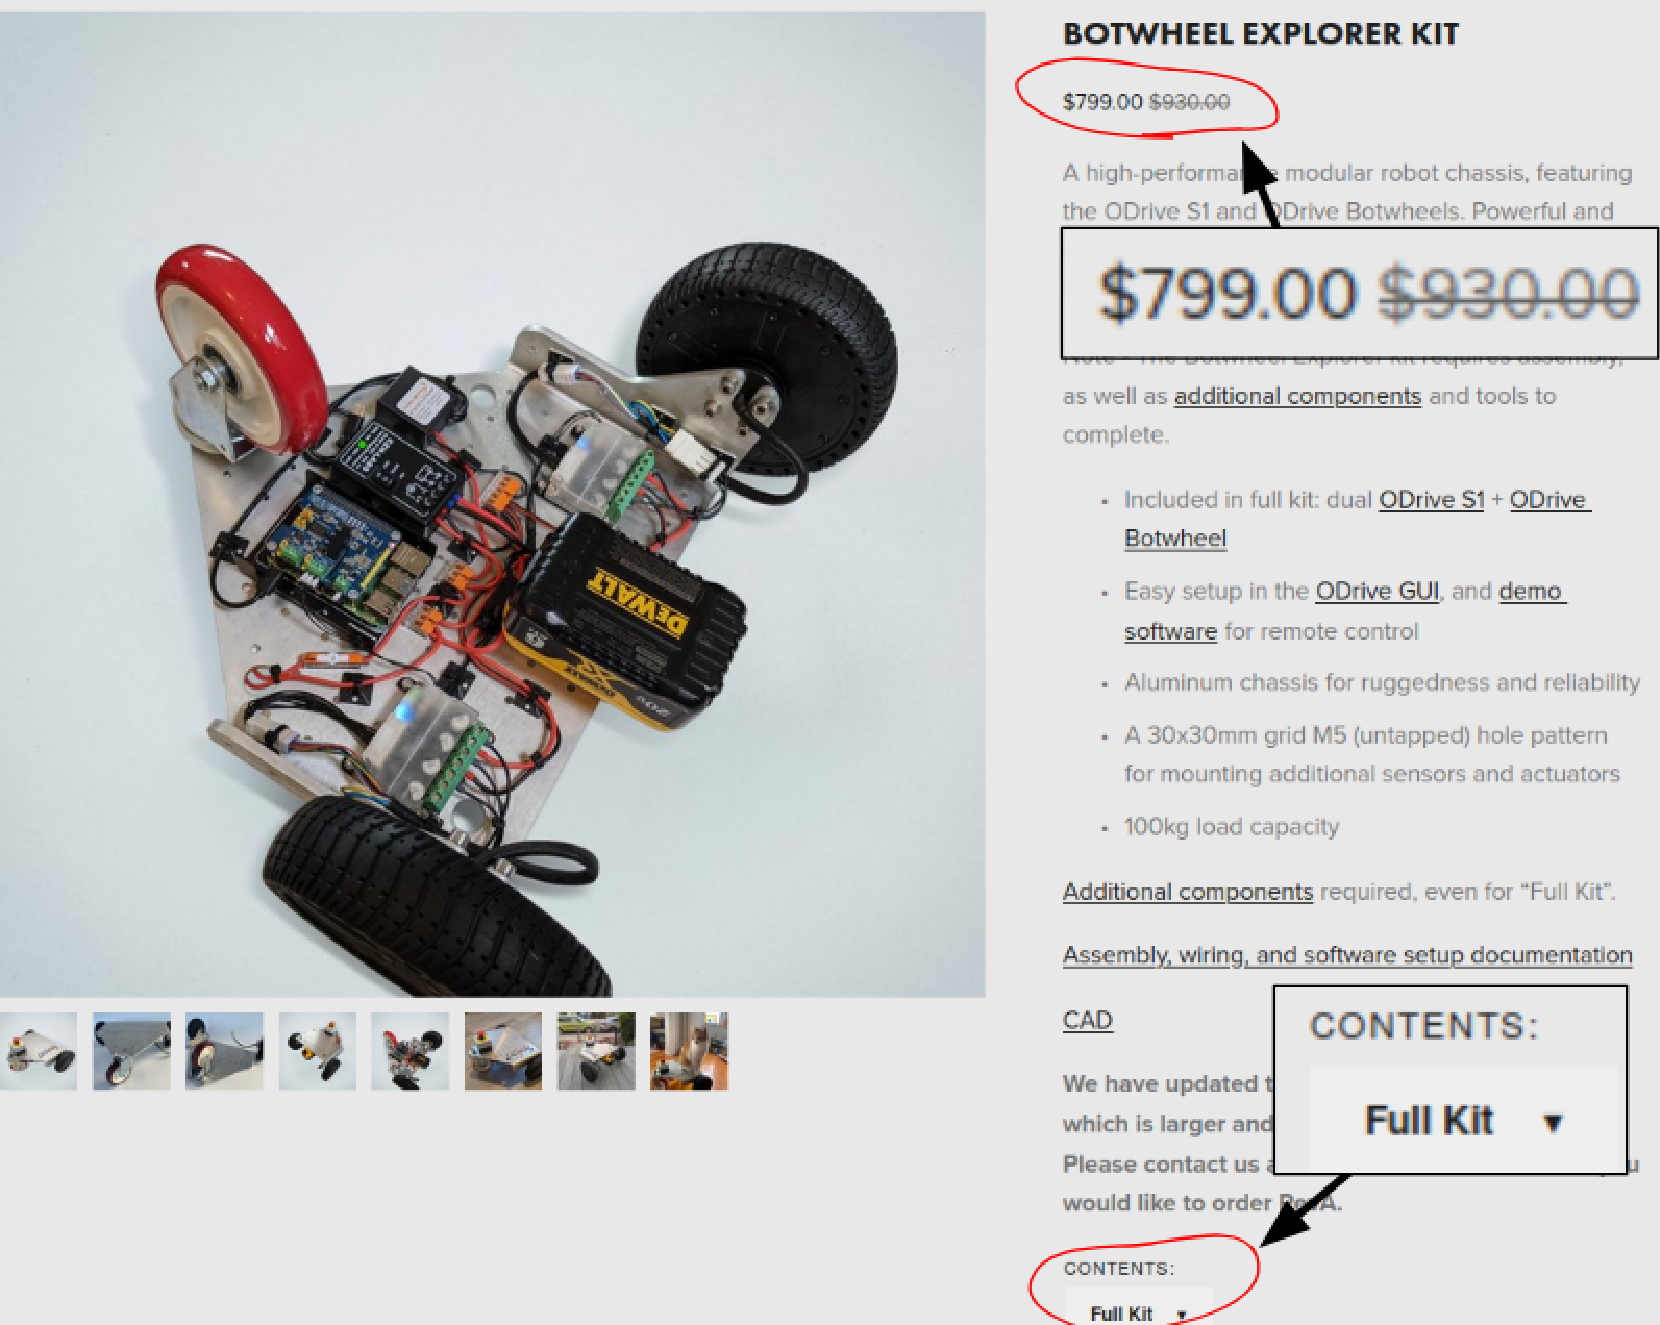
\includegraphics[width=0.8\linewidth]{figs/b_kit_price.pdf}
    \caption{BotWheel Explorer Kitの金額および内容について}
    \label{fig:b_robot_price}
  \end{center}
\end{figure}

このロボットをベースに使用する理由はなんといっても安さである。図\ref{fig:b_robot_price}のように、驚くべきことに\$799で購入することが可能である。
さらに、購入内容としては「Full Kit」という魅力的な内容である。
これは他のロボットの購入サイトを比較しても、類を見ないものであるため、ありがたく購入をさせていただいた。
しかし、「Full Kit」といっても、図\ref{fig:b_robot_price}のような電装部品も込みというわけではなかった。
商品ページの画像にはいかにも全て揃っているように間違える可能性があるので注意する必要がある。
また、購入のタイミングでは円相場と海外手数料について考慮する必要がある。

Full Kitを購入した場合に梱包されているものを表\ref{tab:botwheel_kit}に示す。
内容としては、駆動用のインホイールモータ、制御用のモータドライバ、
モータの取り付けおよび機体のボーディのためのシャーシ、モータドライバとインホイールモーター間の通信に必要な
CANハーネスが梱包等が梱包されている。
\begin{table}[h]
  \centering
  \begin{tabular}{|l|c|l|}
      \hline
      \multicolumn{3}{|c|}{\textbf{BotWheel Explorer Kit(Full Kit)}} \\
      \hline
      部品 & 数量 & 詳細 \\
      \hline
      ODrive S1 & 2 & モータドライバー \\
      ODrive Botwheel & 2 & インホイールモーター \\
      Chassis Plate & 1 & シャーシ \\
      Caster & 1 & キャスター \\
      CAN harnesses & 2 & CAN ハーネス \\
      \hline
  \end{tabular}
  \caption{BotWheel Explorer Kit の部品一覧}
  \label{tab:botwheel_kit}
\end{table}


BotWheel Explorer Kitは、前方の2つの駆動輪と後方の1つの受動輪が、三角形の金属板に取り付けられている足回りだけのユニットであり、全面の保護カバーはない。
そこで、図\ref{fig:trainee_flame}(a)のように20×20[mm]のアルミフレームを金属板に固定し、(b)に示すようにポリプレートのカバーを取り付けることで雨除けとした。
ポリプレートは、厚さ3[mm]で、手で簡単に曲げられることから湾曲した形状を作りやすいため採用した。
さらに、金属板にはナットが飛び出ている箇所があるなど平らなスペースが小さいことから、アルミフレームの上に四角形のポリカーボネート\cite{PE960_1}の板を取り付け、ノートPCやバッテリーを搭載できるスペースを広げた。
また、ロボットの最低高さ600[mm]という寸法制限と運搬のしやすさを考え、アルミフレームを上部に伸ばし台車の持ち手のような構造とした。
非常停止スイッチ・3次元LiDARは、3Dプリンタで治具を製作しアルミフレームに固定した。
%また、手動操作用のコントローラー置き場・信号検出用のスマートフォン置き場も、3Dプリンタで製作しアルミフレームに取り付けた。\par

アルミフレームや治具等の設計には、Fusion360\cite{Fusion360}を使用した。
ただ、無料ライセンスではチーム開発ができなかったため、制作したCADモデルを共有する際にはOnshape\cite{Onshape}を使用した。


センサ構成について、図\ref{fig:botwheel-explorer-schematic}に示す。
\begin{figure}[h]
  \begin{center}
    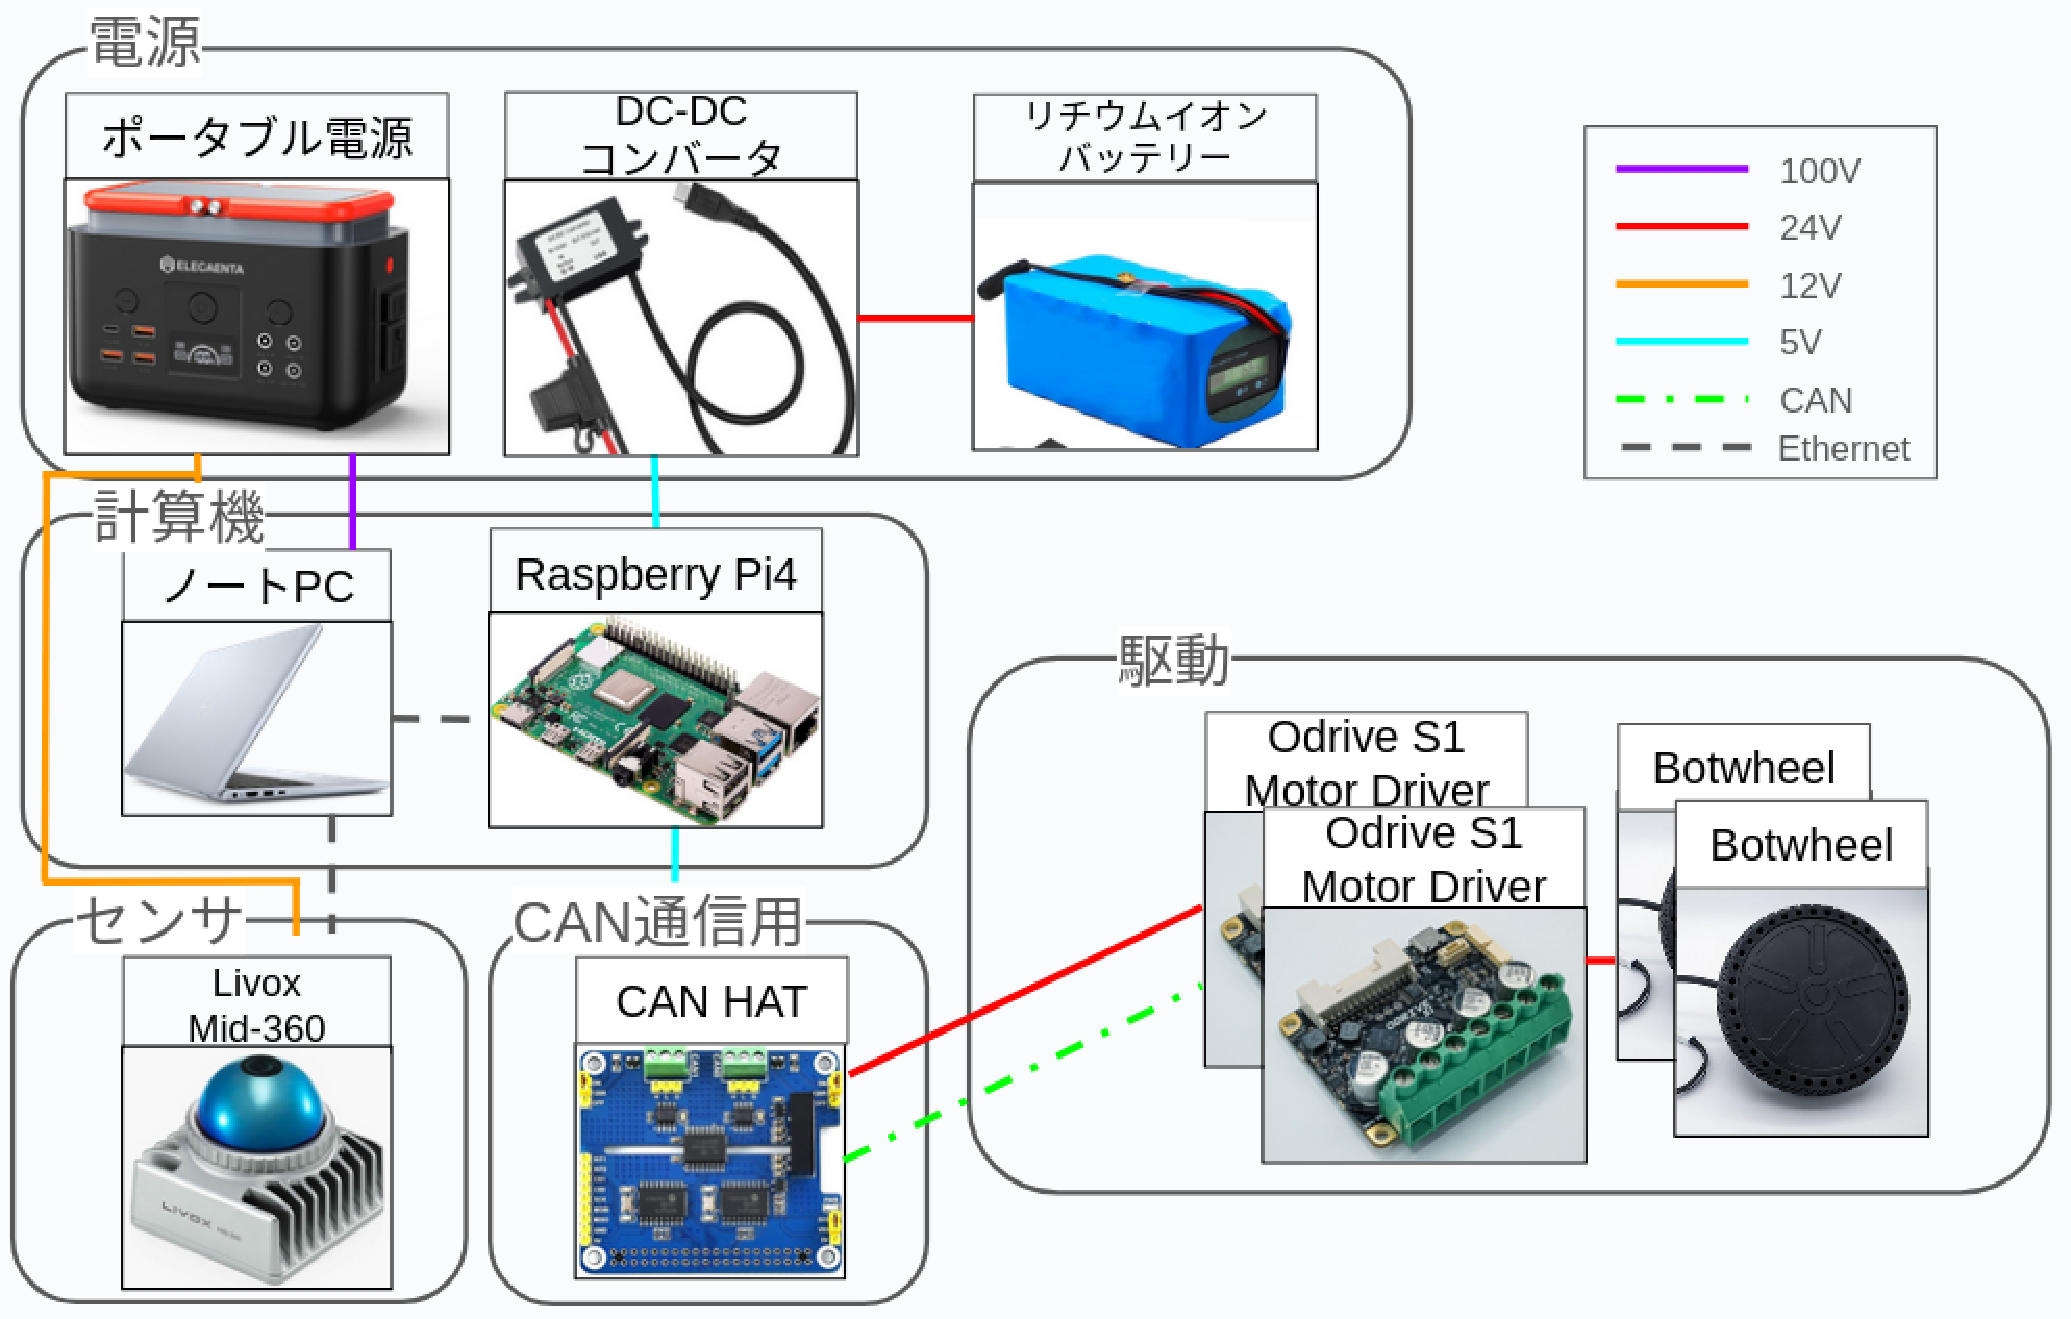
\includegraphics[width=1.0\linewidth]{figs/botwheel-explorer-schematic.pdf}
    \caption{機体の回路構成}
    \label{fig:botwheel-explorer-schematic}
  \end{center}
\end{figure}

センサーについては、3次元LiDARとIMUが内蔵されているLivox社のMid-360を搭載した。
Mid-360を採用した理由は下記の4点である。

\begin{itemize}
  \item[1] 本走行エリアでの使用を想定した際に、測定可能な距離が十分に長いこと
  \item[2] 一つのLiDARで360[deg]の測定が可能であること
  \item[3] 安価であること
  \item[4] IMUが内蔵されていること
\end{itemize}

Mid-360の取り付け位置は、1つのLiDARで自己位置推定と障害物回避が両立できることを目標として設計した。
自己位置推定は植木などを検知しながら地面の勾配などの影響を受けないようにするために、
地面から高さ10〜30[cm]付近の3次元点群を2次元に変換することで行う。
また障害物回避は地面周辺が死角とならない範囲が広いほど軌道計画を柔軟に行うことができる。
そのため、地面から高さ10〜30[cm]付近の点群を測定できる条件下で前述の機体を覆うカバーによって生まれる
死角をできる限り狭くするために、図\ref{fig:trainee_flame}(b)に示す通り下向きにLiDARを取り付ける方針とした。
なお機体を覆うカバーによって生まれる死角はOnshapeの3Dスケッチ機能を用いて描画し、
より死角の少なくなる取り付け位置を算出した。

% 計算機については、ノートPCを各ロボットに搭載して使用した。
% ?ここいる or 要訂正?
% 昨年は、1チームが計算機としてRaspberry Pi 4 Model Bのみを
% 使用して自律走行を実現した\cite{池邉2022}。
% しかし本年度については、
% Raspberry Pi上でROS 2を実行するための
% 技術的な課題が解決しておらず、
% ノートPCを使用することとなった。
% この場合、Raspberry Pi Catには、
% ノートPCと制御用のRaspberry Piの2台の計算機が搭載されることとなる。
% センサ構成としては、各チームの機体に外界センサとして
% 2次元LiDAR、3次元LiDAR、内界センサとしてIMUを搭載した。
% ?ここいる or 要訂正?

\begin{figure}[h]
  \begin{center}
    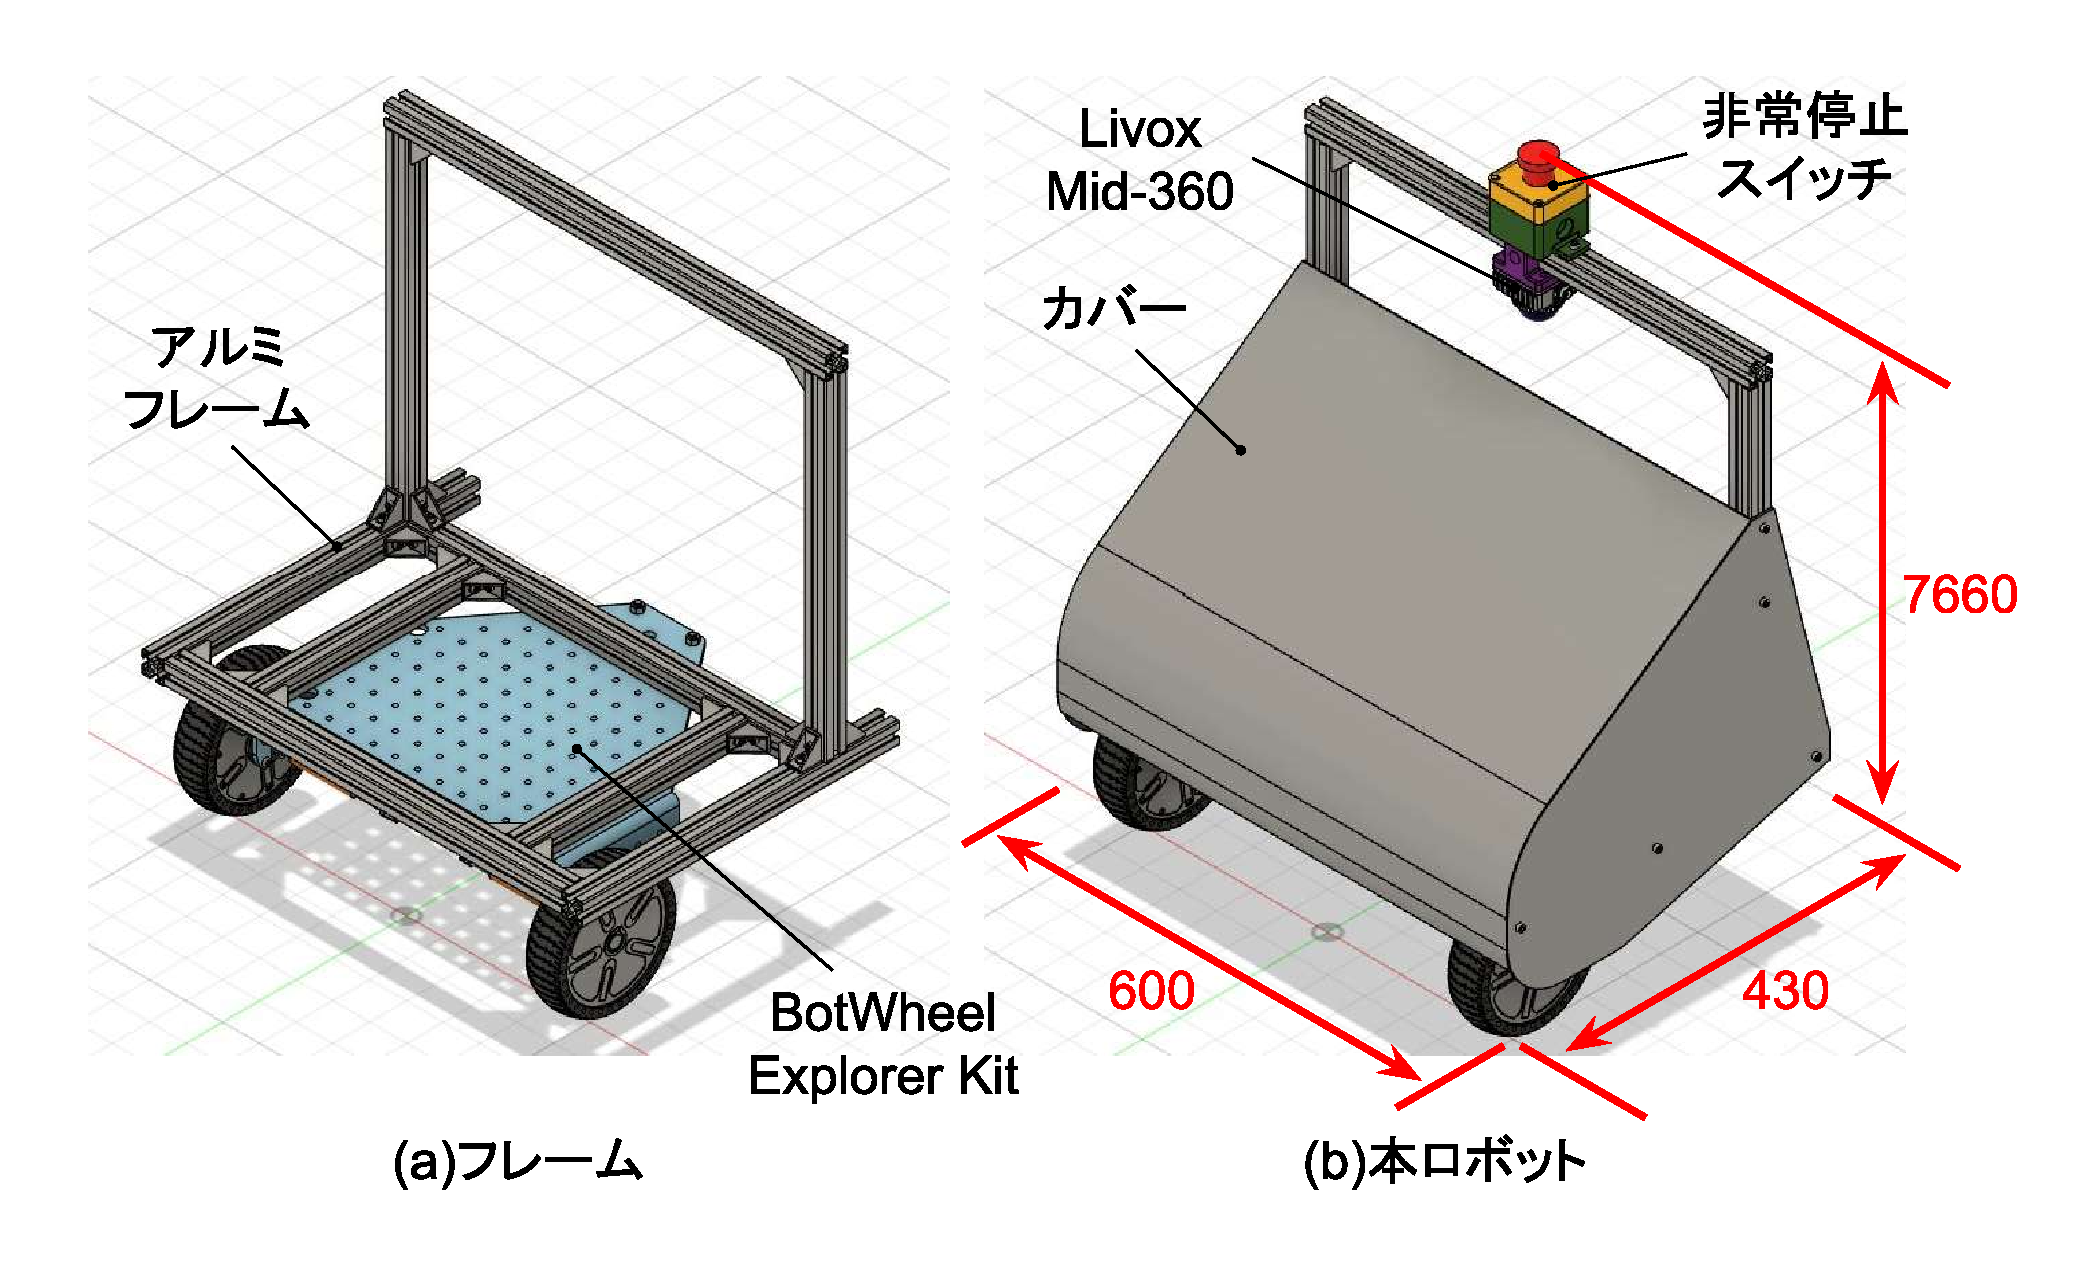
\includegraphics[width=1.0\linewidth]{figs/robot_flame.pdf}
    \caption{メカ設計}
    \label{fig:trainee_flame}
  \end{center}
\end{figure}

\subsection{ソフトウェア構成}\label{sub:software}

本チームで用いたソフトウェアはすべて、Ubuntu 22.04上で動作する
既存のROS 2 Humble用のパッケージを使用した。
使用したパッケージはGitHub上に公開されているため、誰でも使用することが可能である。
また,ソフトウェア開発環境をチームで統一するためにDocker上でROS 2 Humble環境を構築した.

本チームのシステムの構成を図\ref{fig:shinsotu_system_diagram}に示す.
ロボットに搭載された3D LiDARからセンサ情報をノートPCに送信する.
ノートPCは自己位置推定,経路生成,経路追従などの主要となる計算を行う役割を担当した.
これらの計算結果から得られた制御指令がRaspberry Pi 4Bに返される。

\begin{figure}[h]
  \begin{center}
    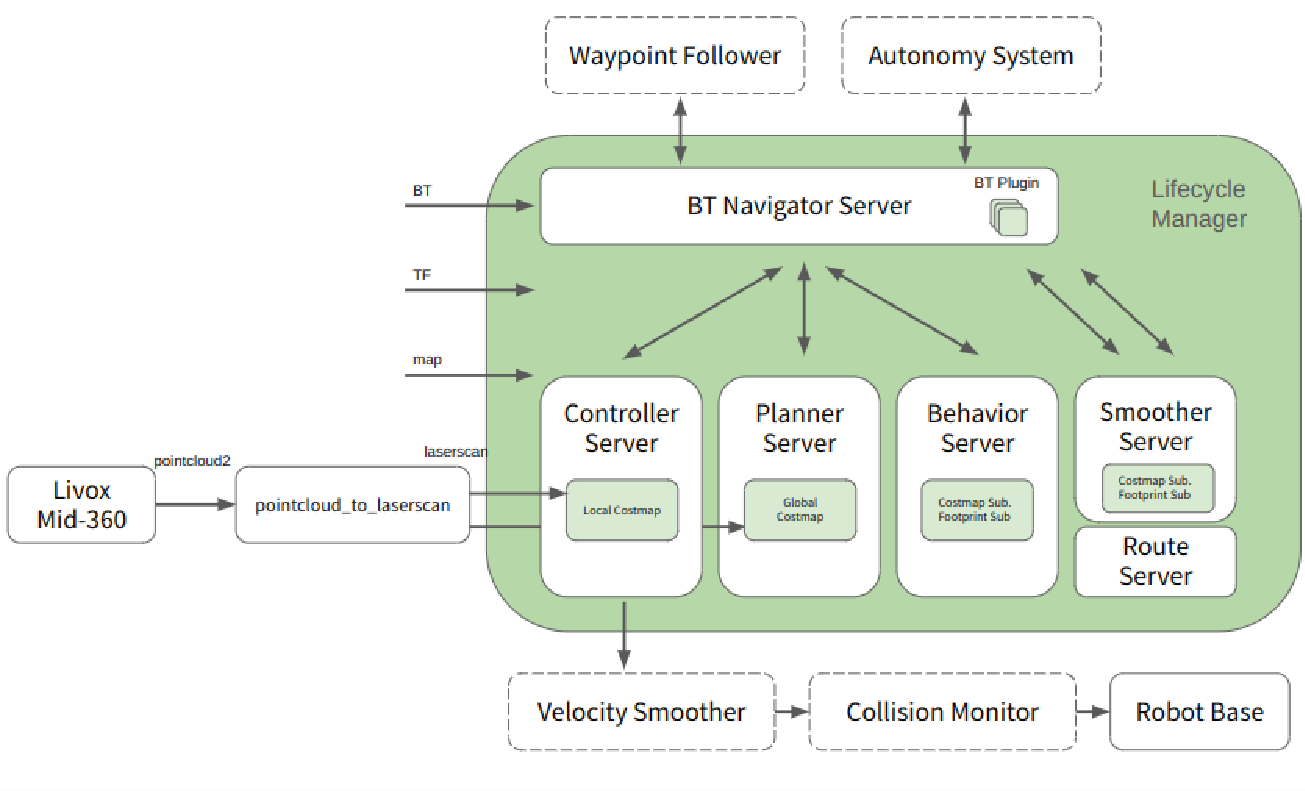
\includegraphics[width=1.0\linewidth]{figs/shinsotu_system_diagram.pdf}
    \caption{システム構成 \cite{nav2_docs}}
    \label{fig:shinsotu_system_diagram}
  \end{center}
\end{figure}


\subsubsection{自律移動システム}

自律移動の手法は、3D LiDARから取得した走行区間のスキャンデータから2次元の環境地図を事前に作成し、
実際のロボット走行中に取得するスキャンデータとのマッチングにより求めた自己位置をもとに自律走行を行うものである。
2次元地図の作成には2次元のレーザースキャン情報が必要となる。
今回使用したLiDARから得られるスキャンデータは3次元点群であるため2次元に変換する処理を行った。
3次元点群から2次元のレーザースキャン情報への変換には、pointcloud\_to\_laserscan\cite{pcl_lsc}を使用した。

自己位置推定には,navigation2の自己位置推定パッケージである
nav2\_amclを使用した\cite{nav2_amcl}.
経路計画と障害物回避には,Nav2を使用した\cite{nav2}.
経路計画は2次元環境地図上で実行され,推定したロボットの位置($xy$座標)と向き($z$軸周り)の情報から計算される.
その際,必要になった2次元環境地図の作成にはslam\_toolbox\cite{slam_toolbox}を使用した.
なおamclを用いたため、Mid-360のIMUは使用しなかった。

\section{本走行・実験走行の結果}
\subsection{本走行の結果}

つくばチャレンジ2024での本走行の結果を表\ref{MainRun}に示す。

\begin{table}[H]
  \caption{各チームの本走行の結果}
  \label{MainRun}
  \begin{tabular}{|c|c|p{4.0cm}|}
    \hline
    走行距離 & リタイアの理由                                                                                             \\
    \hline
    % 429[m]   & 目標である確認走行区間完走を達成したため                                                           \\
    429[m]   & 確認走行区間以降の地図が未取得であったため                                                           \\
    \hline
  \end{tabular}
\end{table}

% 本走行の結果は表の通り、確認走行区間を完走して終了を申告したため、
本走行の結果は表の通り、確認走行区間を完走して終了を申告したため、
429[m]という結果になった。
本チームの目標である確認走行区間の完走を達成することができたものの、
% 確認走行区間より先の区間については今年度のメインターゲットではなく、
その目標に注力したため、それ以降の区間の地図が完成できず、本走行を継続できなかった。
% その目標に注力したため、それ以降の区間の自己位置推定に使用する地図の作成が完了せず、本走行を継続できなかった。

\subsection{本走行・実験走行で見つかった課題}

本チームは、10/6、10/26、10/27、11/9、11/10、11/25、12/6、12/7、12/8の計9日間、実験走行および本走行に参加した。
これらの走行で見つかった課題を以下に挙げる。
\subsubsection{地図と実際の環境との違い}
実験走行において、スタート地点付近で自己位置をロストしてしまうという課題があった。
この課題は、テントの設置場所などの変化により市役所の壁が遮られ、点群が更新されるたびに
自己位置の尤度が下がっていくことが原因であると考えたため、
% 点群の更新頻度を下げることで解消した。
点群の更新を高頻度で行うことで対処した。
具体的にはamclのパラメータのうち、update\_min\_aを0.1に、update\_min\_dを0.125とデフォルト値の半分に変更した。

\subsubsection{グローバルプランナーの経路選択}
本チームが使用したグローバルプランナーは、地図上にある障害物や侵入可能領域外との境界からできるだけ離れたルートを選択する。
これにより、市役所裏側の道路では障害物が少ないため、道路の中心を走行してしまうという課題があった。
この課題は地図上の侵入可能領域を狭くし、道路の端しか通ることができないようにすることで解消したが、
侵入可能領域を狭くすることは自己位置ロストのしやすさとトレードオフの関係にある。
そのため、今後はグローバルプランナーの調整により障害物からできるだけ離れるような
経路選択を行わせないようにすべきであると考えられる。

% \subsubsection{旋回によるオドメトリのずれ}
\subsubsection{旋回量のずれ}
確認走行区間を超えた先の地図づくりを行う中で、回転量がずれてしまうという課題があった。
この課題は現時点では解消することができていないが、ヨー方向のずれが大きいことから
IMUの情報を組み合わせて推定することにより解消できると考えられる。

\subsubsection{3次元点群の抽出高さ}
実験走行の中で、車止めを検知することができず衝突してしまうという課題があった。
これは3次元点群を2次元に切り出す高さのパラメータチューニングにより解消したが、
3次元点群を2次元に切り出す高さを低くすることは、地面勾配へのロバスト性とトレードオフの関係にある。
そのため、今後これらのトレードオフを解消できるような地面と障害物を区別するようなロジックが必要であると考えられる。

\section{その他の試み}
本章では、自律走行時において未実施である、
選択課題B信号認識横断についての取り組みの取り組みついて紹介する。
\\ 本年度は確認走行区間の達成であったが、今後選択課題に挑戦することを見据えて信号認識横断の課題を取り組んだ。
本課題を選択した理由は、ロボットの機体がその場になくてもデータ収集と手法確認を行え、個別に開発を進められるためである。
\\ 本課題では、日の当たり方が大きく異なる信号をミスなくかつ素早く検出することが求められる。
そのためカメラはホワイトバランス調整などが行えるものであり、
加えて、チームの目的も踏まえると安価であることが好ましい。
そこでカメラにはスマートフォンを採用した。
一般的なスマートフォンには上記の機能が備わっており、旧型モデルを用いることで価格も抑制できる。
本チームでは図\ref{fig:smartphone}に示す2020年発売のGalaxy A21 SCV49を採用した。
\\ 本課題を達成するには、歩行者用信号(以下、信号)の検出の他に横断歩道内で停止している自動車の有無の確認などの安全確認が求められる。
この問題に対して深層学習による物体認識を用いることで対処する。
物体認識に用いる学習済みモデルは、VIDVIP\cite{BabaVIDVIP}が提供している,vidvipo\_yolov8nとした。
このモデルは、交通認識に特化したものである。認識結果の例を図\ref{fig:result_yolo}に示す。
自動車や横断歩道、赤色の歩行者用信号などから、低木などの周辺環境まで認識できていることが確認できる。
歩行者信号に対して追加学習の必要がなく、かつYOLOv8であるため認識が比較的高速である。
\\ 
このモデルに対して、事前に取得した課題コース上から撮影した動画を認識させたところ、青信号が検出できない場合が存在することを確認した。
そこで、赤信号はYOLOによって発見し、赤信号から青信号への切り替わりは、信号の上部分の赤領域と、下部分の青部分の明度を比較することで対処した。
\\ 今年度は、信号の動画取得と、GPUを搭載したノートパソコン上で動作確認を行った。
来年度では実機への搭載を目指し、電力消費量の少なくなるように手法の軽量化を行うとともに、多様な環境での安定認識などの課題解決に取り組む予定である。
また、スマートフォンのディスプレイを活用し、ロボットの状態表示や一時停止の解除機能も合わせて開発を行いたい。

\begin{figure}[h]
  \begin{center}
    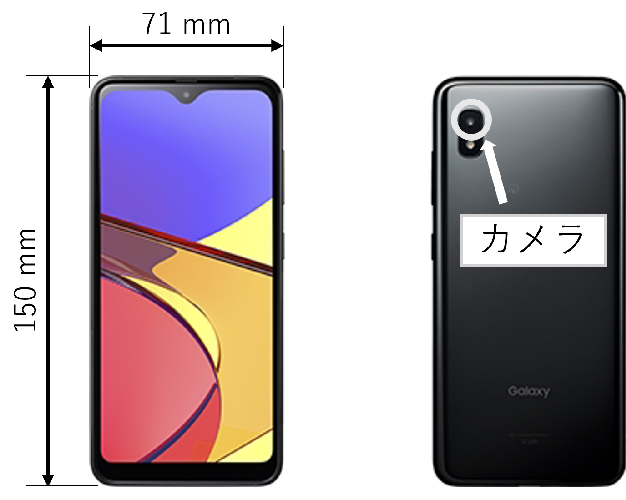
\includegraphics[width=0.6\linewidth]{figs/smartphone.pdf}
    \caption{使用したカメラの外観}
    \label{fig:smartphone}
  \end{center}
\end{figure}

\begin{figure}[h]
  \begin{center}
    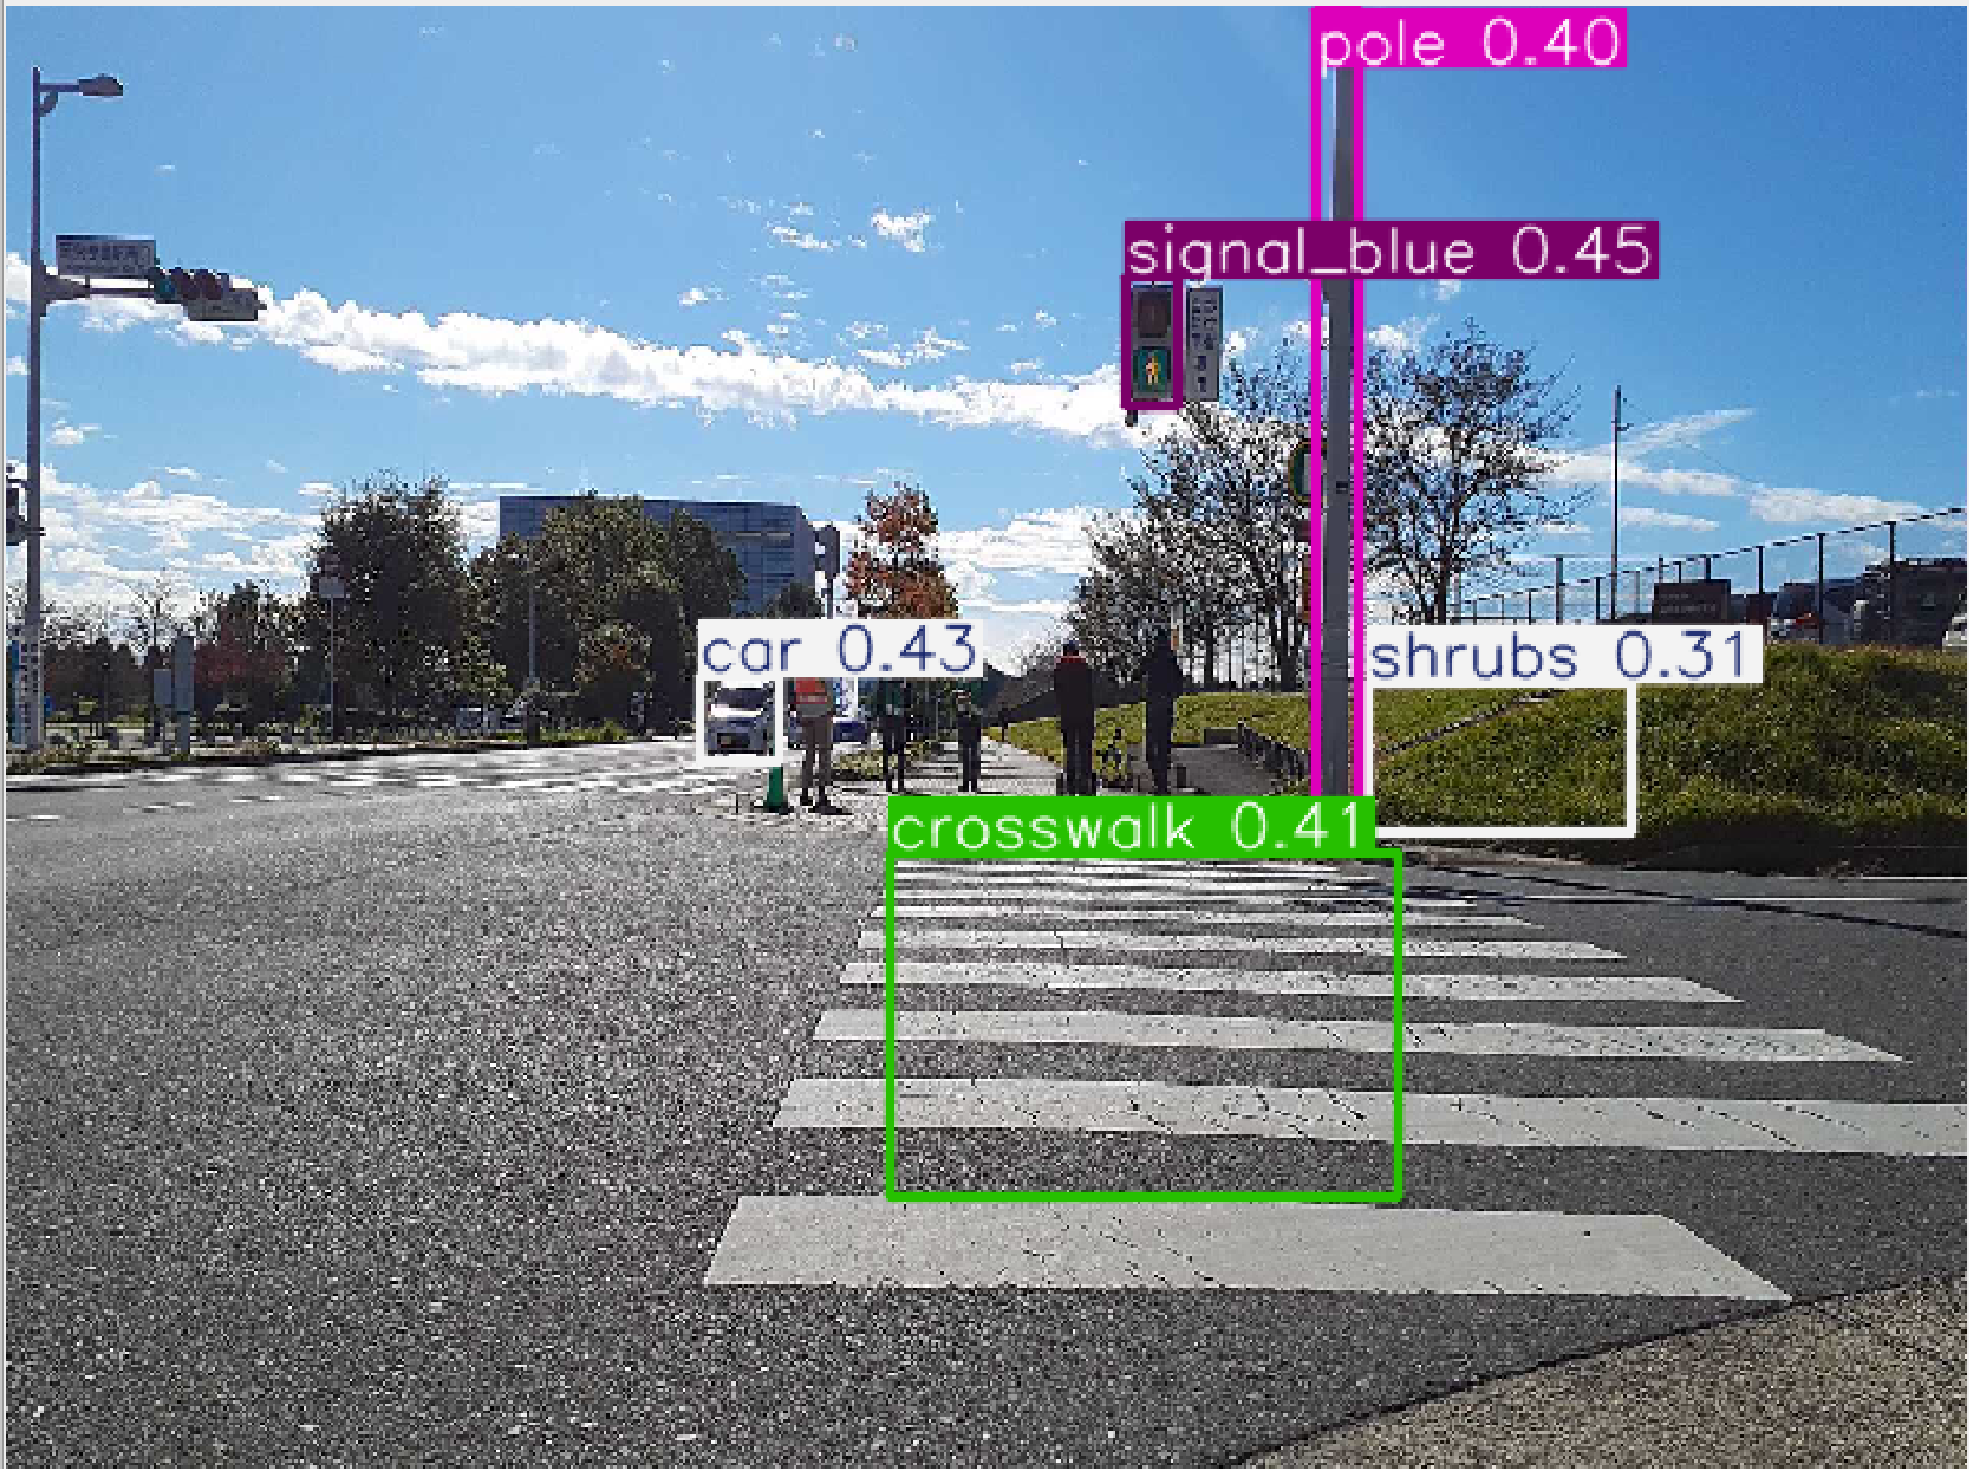
\includegraphics[width=0.6\linewidth]{figs/result_of_yolo.pdf}
    \caption{VIDVIP提供モデルによる認識の例}
    \label{fig:result_yolo}
  \end{center}
\end{figure}
\newpage
\section{結言}
センサとしてLiDAR,IMUを搭載した小型ロボットでつくばチャレンジに参加した.
今回はROSのサポート終了に伴い,
ROS 2に移行したソフトウェア構成で参加した。それに加え、
IMUや3次元LiDARの追加,自作のナビゲーションスタックの使用など,
例年とは異なる試みをした。
来年度は今年度の開発内容をもとに,見つかった課題への対策や,
今回開発が間に合わなかった機能の追加をし,
小型ロボットでのコースの完走を目指す.


\section*{謝辞}
つくばチャレンジ実行委員会,つくば市の皆様に感謝申し上げます.
また上田研究室の皆様には,つくばチャレンジ 2024の参加にあたり、物品の貸与などでご協力頂き感謝申し上げます.
% 上田研究室の新井亮大氏、登内リオン氏,松井大和氏,山崎政光氏,林原研究室の皆様には,つくばチャレンジ 2023の参加にあたりご意見,ご協力頂き感謝申し上げます.
%↑上田整理。あと、著者に名前を連ねない人がいたらここに書くと良いです。

% 参考文献
% \small
\footnotesize
\begin{thebibliography}{99}

  \bibitem{ROS 2}
  Macenski, Steven {\it et al.}: ``Robot Operating System 2: Design, architecture, and uses in the wild,''
  Science Robotics, Vol. 7、No. 66, 2022.

  % \bibitem{emcl2}
  % Ryuichi Ueda: ``ryuichiueda/emcl2,'' \url{https://github.com/ryuichiueda/emcl2} (last visit: 2024-01-01).

  % \bibitem{emcl2_ros2}
  % Ryuichi Ueda: ``CIT-Autonomous-Robot-Lab/emcl2\_ros2,'' \url{https://github.com/CIT-Autonomous-Robot-Lab/emcl2_ros2} (last visit: 2024-01-01).

  \bibitem{PE960_1}
  モノタロウ: ``ポリプレート'',\url{https://www.monotaro.com/p/3576/7697/?} (last visit 2025-01-05)

  \bibitem{RTshop}
  株式会社アールティ: ``Raspberry Pi Cat 屋外でも動かせる中型2輪ロボット'',
  RT Robot Shop Products,\url{https://rt-net.jp/products/raspberry-pi-cat/} (last visit 2024-01-05)

  \bibitem{池邉2022}
  池邉 龍宏,内田 璃空,畑中 優一郎,臼井 温希,庄司 史門,松井 大和,山崎 政光,登内 リオン,林原 靖男,上田 隆一: Raspberry Pi のみを計算に用いる小型移動ロボットでのつくばチャレンジ 2022 参加レポート,つくばチャレンジ2022シンポジウム予稿集,2022.

    \bibitem{ROS}
  Morgan Quigley {\it et al.}: ``ROS: an open-source Robot Operating System,''
  Open-Source Software workshop of the International Conference on Robotics and Automation、2009.

  \bibitem{Fusion360}
  Autodesk,\url{https://www.autodesk.com/jp/products/fusion-360/overview?term=1-YEAR&tab=subscription#top} (last visit 2025-02-02)

  \bibitem{Onshape}
  PTC,\url{https://www.onshape.com/en/} (last visit 2025-02-02)

  %\bibitem{fox2003}
  %Dieter Fox:
  %``Adapting the Sample Size in Particle Filters Through KLD-Sampling,''
  %International Journal of Robotics Research、Vol. 22、No. 12、pp. 985-1003、2003.

  %\bibitem{gutmann2002}
  %Jens-Steffen Gutmann and Dieter Fox:
  %``An Experimental Comparison of Localization Methods Continued,''
  %Proc. of the IEEE/RSJ International Conference on Intelligent Robots and Systems (IROS),pp. 454-459、2002.

  % \bibitem{ueda2002tdp}
  % 	Ryuichi Ueda {\it et al.}: 
  % ``Team description of Team ARAIBO,'' 
  % Proc. of 2002 International RoboCup Symposium、2002. 

  % \bibitem{ueda2004iros}
  % Ryuichi Ueda {\it et al.}: 
  % ``Expansion Resetting for Recovery from Fatal Error in Monte Carlo Localization -- Comparison with Sensor Resetting Methods,'' Proc.of IROS,pp.2481--2486,2004.

  % \bibitem{map2gazebo}
  % Shiloh Curtis: ``shilohc/map2gazebo'',\url{https://github.com/shilohc/map2gazebo} (last visit: 2021-12-31).

  % \bibitem{move_base}
  % Eitan Marder-Eppstein: ``move\_base,'' \url{http://wiki.ros.org/move_base} (last visit: 2021-12-31).

  %\bibitem{amcl}
  %Brian Gerkey: ``amcl,'' \url{https://wiki.ros.org/amcl} (last visit: 2021-12-31).

  %\bibitem{gmapping}
  %Brian Gerkey: ``gmapping,'' \url{http://wiki.ros.org/gmapping} (last visit: 2021-12-31).

  % \bibitem{GIMP}
  % GIMP.org: ``GIMP,'' \url{https://www.gimp.org/} (last visit: 2021-12-31).



  %\bibitem{raspicat}
  %Ryuichi Ueda and Daisuke Sato: ``ja/raspicat,'' \url{https://wiki.ros.org/ja/raspicat} (last visit: 2021-12-31).

  %\bibitem{youtube}
  %BEIKE: ``つくばチャレンジ2022 実験走行 11/19 スタートからゴールまで自律移動(神の手4回),'' \url{https://www.youtube.com/watch?v=3gpjVhRIJDY} (last visit: 2022-12-12).

  % \bibitem{raspicat_rosbag}
  % Tatsuhiro Ikebe: ``uhobeike/raspicat\_rosbag,'' \url{https://github.com/uhobeike/raspicat_rosbag} (last visit: 2021-12-31).

  %\bibitem{池邉2021}
  %池邉 龍宏,曹 越,高橋 秀太,クルス ペレス アントニオ,林原 靖男,上田 隆一: 小型移動ロボットによるつくばチャレンジへの挑戦,第22回計測自動制御学会システムインテグレーション部門講演会,pp.3390-3393,2021.

  

  % \bibitem{上田2019}
  % 上田 隆一: ``詳解確率ロボティクス''、講談社、2019.

  %   \bibitem{上田2020}
  %  上田隆一,鈴木勇矢: 自己位置が不確かな状況における移動ロボットの危険回避行動の生成,第38回日本ロボット学会学術講演会予稿集,pp.RSJ2020AC2C2-02,オンライン開催,2020.

  % \bibitem{地図合成}
  % 川合隆太他: ``産業技術大学院大学における自律移動ロボット「産技大2号」の開発'',2019年度つくばチャレンジシンポジウム、pp.4-7、2020.


  % \bibitem{aws2020}
  %   CIT自律ロボット研究室: ``AWSロボットデリバリーチャレンジで本研究室メンバーが優勝,'' \url{https://lab.ueda.tech/?post=20200915_aws_challenge} (last visit 2022-01-04)

  % \bibitem{学科サイト}
  %   千葉工業大学先進工学部未来ロボティクス学科: ``AWS Robot Delivery Challenge 2021 準優勝''、\url{https://www.robotics.it-chiba.ac.jp/j/?p=838} (last visit 2022-01-04)

  % \bibitem{つくばチャレンジロボット仕様}
  % つくばチャレンジ実行委員会事務局:``つくばチャレンジ 2021 ロボット仕様条件'',
  % \url{https://tsukubachallenge.jp/2021/regulations/specs} (last visit 2021-12-31)

  % \bibitem{UST-30LX}
  % 北陽電機株式会社: ``UST-30LX'',\url{https://www.hokuyo-aut.co.jp/search/single.php?serial=195#spec} (last visit: 2021-12-31).

  % \bibitem{Turtlebot3 Burger}
  % 株式会社ロボティズ: ``Turtlebot3 Burgerの仕様'',\url{https://emanual.robotis.com/docs/en/platform/turtlebot3/features/} (last visit: 2022-1-3).

  % \bibitem{つくばチャレンジ公式記録}
  % つくばチャレンジ実行委員会事務局:``つくばチャレンジ2021の走行結果'',
  % \url{https://tsukubachallenge.jp/2021/records/final} (last visit 2021-12-31)

  % \bibitem{出野畑中}
  %   畑中 優一郎,出野 廣太郎,上田 隆一:``Raspberry Pi 3BのみでRaspberry Pi Catのナビゲーション(屋内環境編)'',CIT自律ロボット研究室,\url{https://lab.ueda.tech/?post=20211210} (last visit 2022-01-02)

  % \bibitem{ike_nav}
  % Tatsuhiro Ikebe: ``uhobeike/ike\_nav,'' \url{https://github.com/uhobeike/ike_nav} (last visit: 2024-01-10).

  % \bibitem{ike_nav_detail}
  % 池邉龍宏: ``自作ナビゲーションスタックでつくばチャレンジ2023に挑戦してみた話'',
  % \url{https://qiita.com/BEIKE/items/f3ff141cc25d49c01363} (last visit 2023-1-10).


  % \bibitem{fox1999etal}
	%   D. Fox {\it et al.}: ``Monte Carlo Localization: Efficient Position Estimation for Mobile Robots,''
  % Proc. of AAAI, pp. 343-349, 1999.

  % \bibitem{hart1968}
  % Peter E. Hart and Nils J. Nilsson and Bertram Raphael: ``A Formal Basis for the Heuristic Determination of Minimal Cost Paths,''
  % IEEE Transactions on Systems Science and Cybernetics, Vol. 4, No.2, pp. 100-107, 1968.

  %\bibitem{dijkstra1959}
  %E. W. Dijkstra : ``A Note on Two Problems in Connexion with Graphs,''
  %Numerische Mathematik, Vol. 1, pp. 269-271, 1959.

  % \bibitem{alberto2006}
  % Bemporad, Alberto: ``Model Predictive Control Design: New Trends and Tools,''
  % Proceedings of the 45th IEEE Conference on Decision and Control, pp. 6678-6683, 2006.

  \bibitem{pcl_lsc}
  ROS Perception: ``ROS Perception/pointcloud\_to\_laserscan (humble branch),'' \url{https://github.com/ros-perception/pointcloud_to_laserscan} (last visit: 2025-02-01).

  % \bibitem{autoware}
  % The Autoware Foundation: ``autowarefoundation/autoware.universe,'' \url{https://github.com/autowarefoundation/autoware.universe.git} (last visit: 2023-11-19).
  
  \bibitem{nav2_amcl}
  ROS Navigation: ``navigation2/nav2\_amcl,'' \url{https://github.com/ros-navigation/navigation2/tree/main/nav2_amcl}  (last visit: 2025-02-02).

  \bibitem{nav2}
  ROS Navigation: ``ros-navigation/navigation2 (humble branch),'' \url{https://github.com/ros-navigation/navigation2} (last visit: 2025-01-30).

  \bibitem{slam_toolbox}
  Steve Macenski: ``slam\_toolbox (ros2 branch),'' \url{https://github.com/SteveMacenski/slam_toolbox} (last visit: 2025-02-01).

  % \bibitem{ike_nav_loc_youtube}
  % 池邉龍宏: ``自作パッケージで屋外自律移動してみた in つくばチャレンジ2023(本走行)'',
  % \url{https://www.youtube.com/embed/k9yxRKOCa14?si=c7ISmE1wH5W4BhgU&amp;start=1365} (last visit 2024-01-05)

%   \bibitem{上田2023}
% 上田隆一, 登内リオン, 池邉龍宏, 林原靖男: ``移動ロボットのための自己位置の不確かさを考慮したセンシングできない固定障害物の回避手法 ---価値反復を用いたナビゲーションにおける状態空間の局所拡張---'', 第28回ロボティクスシンポジア講演論文集, pp. 118-123, 2023.

  % \bibitem{tonouchi2023}
  % 登内リオン, 池邉龍宏, 林原靖男, 上田隆一: ``価値反復を用いた移動ロボットによる屋外ナビゲーション,''
  % 日本機械学会ロボティクス・メカトロニクス講演会, 2P1-G06, 2023.

  % \bibitem{ueda2023JRM}
  % R. Ueda, L. Tonouchi, T. Ikebe, and Y. Hayashibara: ``Implementation of Brute-Force Value Iteration for Mobile Robot Path Planning and Obstacle Bypassing,''
  % J. Robot. Mechatron., Vol.35, No.6, pp. 1489-1502, 2023.

  % \bibitem{ikebeMECH}
  % 池邉龍宏, 林原靖男, 上田隆一: ``未知障害物によるモンテカルロ自己位置推定の破綻を防ぐための観測範囲の制限と選択'',
  % 日本機械学会ロボティクス・メカトロニクス講演会, 2A2-G06, 2023.
  
  \bibitem{BabaVIDVIP}
  T. Baba, “VIDVIP: Dataset for Object Detection During Sidewalk Travel,” J. Robot. Mechatron., Vol.33 No.5, pp. 1135-1143, 2021. https://doi.org/10.20965/jrm.2021.p1135
  
  \bibitem{nav2_docs}
  Nav2 — Nav2 1.0.0 documentation, \url{https://docs.nav2.org/} (last visit: 2025-02-01).
\end{thebibliography}
\normalsize

\clearpage

%\section{付録として、各実験走行でどんなことをやっていたかを書く?}
% 当チームは、9日間分のすべての実験走行会に参加した。
% 7月2日、7月23日は確認走行区間から信号あり横断歩道手前までの自己位置推定のテストを行った。
% 地図は昨年作ったものを使い、自己位置推定のパッケージにemcl2を使った。
% また、駅・公園エリアの地図作成のためのrosbagを取った。
% 9月17日、10月1日は駅・公園エリアの走行実験を行った。
% 走行エリアが増えたことに伴い地図の容量が増大し、4GBメモリのRaspberry Piでは処理できなかった。
% メモリの容量を増やし、地図の余白部分を削ることで駅・公園エリアが走行できるようになった。
% 10月22日、10月23日は信号あり横断歩道の横断の走行テストを行った。
% 通常の走行速度では青信号中に横断しきれなかったため、
% 信号あり横断歩道の横断中のみ走行速度を変えることで、青信号中に横断しきることができた。

\end{document}
